% Appendix of the ICLR 2027 draft (input from main.tex after the bibliography).

\section{The rebuilt corpus, step by step}
\label{app:data}

\paragraph{Counts.}
The original corpus holds 37{,}489 unique sprites (after cutting sheets into connected components at native scale and
dropping glyphs, UI and near-monochrome crops). Native sizes: 710 at most 12\,px, 2{,}675 at most 16\,px, 9{,}687 at
most 20\,px, 12{,}516 at most 24\,px, 19{,}611 at most 32\,px. Exact-pixel hashing finds 4{,}888 duplicate copies;
16.2\% of the 3{,}000 held-out evaluation sprites and 17.0\% of the 200 external-comparison sprites have a
pixel-identical twin that the path-based hold-out leaves in training. Integer-upscaled pixel art, which could be
restored by dividing by its block size, accounts for only 4.6\% of the corpus.

\paragraph{New material.}
The CC-BY-4.0, CC-BY-SA-3.0 and OGA-BY-3.0 OpenGameArt collections (8.8\,GB of 2D art) yield 37{,}226 cut sprites.
Filtering by the same rules removes 8{,}184; cross-corpus pixel hashing removes a further 6{,}062 that duplicate the
existing corpus; a filename filter removes 367 font, UI and text sheets; average-hash collapse of animation frames
removes 3{,}456; a cap of 60 sprites per source sheet removes the rest, leaving 14{,}999 sprites from 1{,}207 sheets.
Verification of this set: median palette 6 colours, 98.2\% of visible pixels fully opaque, mean flat-neighbour fraction
0.434, native sizes 234 / 1{,}726 / 5{,}374 / 6{,}028 at most 12 / 16 / 20 / 24\,px. Every sprite keeps its source zip,
member path and licence in a manifest.

\paragraph{Captions.}
We caption the new sprites with gemini-3.8-flash on numbered $4\times5$ grids of nearest-upscaled sprites on a
checkerboard, one caption per cell, 6--15 words, with an explicit ``unclear abstract shape'' escape. Of 14{,}999
sprites, 14{,}845 receive a caption (99.0\%); dropping the escapes, degenerate strings and 11 rows that echoed the
instruction leaves 13{,}987 usable captions, 99.6\% distinct, median 13 words. We selected the captioner by running the
same grid through ten vision--language models: gemini-3.8-flash parsed all 20 cells in both trials at 22\,s per call and
was the most accurate, while a larger sibling truncated at cell 11 in both trials and several models mislabelled
weapons and buildings.

\paragraph{Training-set composition.}
With duplicates removed and downscaling limited to $1.5\times$, the rebuilt corpus yields 86{,}290 training rows
(12/16/20/24\,px buckets: 7{,}357 / 11{,}733 / 15{,}087 / 17{,}199), against 64{,}990 without the new sprites and
180{,}533 under the original policy, which fed 48\,px artwork to the 16\,px bucket.

\paragraph{Near-duplicate collapse is harmful.}
Collapsing average-hash near-duplicates in the \emph{old} corpus as well (37{,}489 $\to$ 26{,}504 groups) costs more
than it gains: at 20k steps it scores 21.07 biased / 162.23 native against 20.31 / 151.85 for the same recipe without
the collapse. We therefore drop only exact duplicates in the main corpus and apply the collapse only to the new
material, where single sheets contributed up to 563 frames of one character.

\section{Cross-resolution guidance: equations and full tables}
\label{app:crossres}

The cross-resolution rules referenced in Section~\ref{sec:analysis} use the guided prediction
$\tilde e = \eref + w\,(e_{\text{strong}} - \eref)$ with
\begin{equation}
  \eref^{\text{label}} = \epsilon_\theta(x_t, t, c, \blow), \qquad
  \eref^{\text{comp}} = \epsilon_{\theta_{\text{snap}}}(x_t, t, c, \blow), \qquad \blow < b_R,
  \label{eq:ref}
\end{equation}
i.e.\ the same network (or an early EMA snapshot of it) queried under a lower resolution bucket, with $\blow = 12$ at
16\,px and $\blow = 16$ at 20 and 24\,px. The internalised variant follows guidance-free training \citep{Chen2025gft}:
the network gains a scalar input $\beta \in (0,1]$ and is trained with
\begin{equation}
  \hat\epsilon_\beta(x_t, t, c, b) = \beta\,s_\theta(x_t, t, c, b, \beta) + (1-\beta)\,\sg[\epsilon_{\theta_{\text{snap}}}(x_t, t, c, \blow(b))],
  \label{eq:gft}
\end{equation}
so that setting $\beta = 1/w$ at inference reproduces the rule of Eq.~(\ref{eq:ref}) in a single forward pass. The
internalised model is initialised from the base model and trained for 10k further steps (Table~\ref{tab:hparams}).

On the rebuilt model, scored against native pixel art, these rules give 114.9 (label), 117.0 (composed), 178.8
(internalised, $\beta = 1$) and 170.3 (internalised, $w = 1.5$), against 113.2 for CFG 1.0 and 87.1 for ICG; under the
biased reference the internalised model is the best row of Table~\ref{tab:full16} (10.4). The reference is a
lower-resolution belief, so extrapolating away from it adds contrast without reducing the palette, which the biased
reference rewards and the native one does not.

\section{Implementation and protocol details}
\label{app:details}

\begin{table}[h]
\caption{Training and sampling configuration.}
\label{tab:hparams}
\centering
\small
\begin{adjustbox}{max width=\linewidth}
\begin{tabular}{@{}ll@{}}
\toprule
Denoiser & diffusers \texttt{UNet2DConditionModel}, 4 input/output channels (RGBA), widths 128/256/512, \\
 & 2 layers per block; down: CrossAttn, CrossAttn, plain; up: plain, CrossAttn, CrossAttn; 72.5M parameters \\
Text & frozen CLIP ViT-B/32 text encoder, 77 tokens, last hidden states (512-d) as cross-attention context \\
Resolution & class embedding over $\mathcal{B} = \{12,16,20,24,32,48,64\}$ added to the timestep embedding; never dropped \\
Diffusion & $\epsilon$-prediction, $T = 1000$, cosine (\texttt{squaredcos\_cap\_v2}) schedule \\
Base training & from scratch, 80k steps, AdamW, constant lr $5\cdot10^{-5}$, EMA 0.999, caption dropout 10\% \\
Batches & one bucket per batch, bucket drawn proportionally to its row count; batch 320 / 256 / 224 / 192 / 128 / 64 / 40 \\
 & for 12 / 16 / 20 / 24 / 32 / 48 / 64\,px \\
Sampler & ICG $w{=}2$; PPS with $f{=}0.5$, $k{=}8/4/8/6/8$ at 12/16/20/24/32\,px, 8 $k$-means iterations; opaque = $\hat\alpha > 0.5$ \\
Snapshot & 10k-step EMA of an independent 10k-step run with the same recipe (cross-resolution composed reference only) \\
Internalization & init from the base model, 10k steps, same optimizer/lr/EMA/batches; $\beta\sim\mathcal U(0.4,1)$, $\beta{=}1$ w.p.\ 0.25 and for 12\,px rows; \\
 & reference rung 12 (for 16\,px rows) and 16 (for 20 and 24\,px rows); $\beta$ via 256-d sinusoidal embedding of $1000\beta$ \\
 & and a zero-initialized linear map into the timestep features (32,768 parameters) \\
Sampling & 100-step ancestral DDPM, EMA weights, one sample per prompt \\
\bottomrule
\end{tabular}
\end{adjustbox}
\end{table}

\paragraph{Canvas preprocessing.} A sprite larger than the target side $R$ is reduced with a premultiplied-alpha box
filter, preserving aspect ratio; a sprite at most $R/2$ is enlarged by an integer nearest-neighbour factor. It is then
centred on a transparent $R\times R$ canvas, and alpha is thresholded at 128 (pixels below become fully transparent,
with RGB cleared). Generated samples are stored with the same hard alpha. The same function produces the FD reference
set, the held-out floor set and the ``downscale'' external baselines.

\paragraph{Evaluation prompts and training exclusion.} All real sprites of the original corpus are split once with a
fixed shuffle into a 3,000-sprite \emph{biased} reference set and a disjoint held-out pool. The first 3,000 held-out
sprites supply, through their recaptions, the 3,000 evaluation prompts. The biased reference and these 3,000 held-out
sprites (5,928 paths) are removed from training, together with every exact duplicate of them.

\paragraph{Native reference.} The sprites of the original corpus that are natively at most $R$\,px are split in half with
a fixed seed into the native reference and a disjoint floor set (16\,px: 1,337 and 1,338). This pool is not removed from
training except where it overlaps the 5,928 excluded paths; the training-excluded native set of
Section~\ref{sec:analysis} consists of the floor-set sprites that are among the excluded paths (210 at 16\,px).

\paragraph{FD.} Each image is composited on white and resized to $R\times R$ (box filter; generated images are already
$R\times R$). It is then nearest-neighbour upsampled to $224\times224$, normalized with ImageNet statistics, and embedded
by the CLS token of \texttt{facebook/dinov2-small}. FD is the Fréchet distance between Gaussian fits of the two feature
sets (at 16\,px: 3,000 samples vs.\ 1,337 native or 3,000 biased reference images; 200 samples for the external
comparison). Samples are generated in chunks of 1,000 prompts, and chunk $i$ uses seed $s + i$.

\paragraph{CLIP.} The same saved samples are composited on mid-grey, nearest-neighbour upsampled to 224\,px and scored
with CLIP ViT-B/32 against the caption they were sampled from. We report $100\cos$ and R@1, the fraction of samples
whose own caption ranks first among itself and 99 random held-out captions (chance 1\%).

\section{Recaptioning}
\label{app:recap}

\begin{table}[h]
\caption{Caption statistics before and after recaptioning (43,342 unique training and evaluation images).}
\label{tab:recap}
\centering
\small
\begin{adjustbox}{max width=\linewidth}
\begin{tabular}{@{}lcc@{}}
\toprule
 & BLIP \citep{Li2022blip} (original) & gemini-3-flash \citep{Gemini3} (recaptioned) \\
\midrule
Distinct captions & 23.5\% & 98.6\% \\
Words per caption (median / mean) & 8 / 7.6 & 12 / 12.1 \\
Occurrences of the most frequent caption & 7,669 (``a pixel art sprite'') & 6 (``human'') \\
Share of data covered by the ten most frequent captions & $\approx$25\% & $<$0.1\% \\
\bottomrule
\end{tabular}
\end{adjustbox}
\end{table}

Images were sent as numbered grids on a checkerboard (20 per request, 12 for retries). For each cell, the instruction
asked for a caption of 6--15 words that names the object first and then its distinguishing colours, materials and
parts, describes only what is visible, and avoids uninformative words (``pixel art'', ``sprite'', ``8-bit'', ``icon'').
Of the 43,342 unique images, 41,560 received a caption and 41,103 (94.8\%) were usable. The remainder were declared an
``unclear abstract shape'' by the captioner and keep their BLIP \citep{Li2022blip} caption. Across the three caption files (49,652 rows),
95\% of rows were replaced. The total cost was about 18.7M tokens. The held-out evaluation prompts are the recaptions of
the held-out sprites, so the evaluation prompts follow the training caption distribution.

\section{External systems: pipeline and qualitative comparison}
\label{app:externalfig}

The gpt-image-2 \citep{GPTImage2} renders were requested at 1024\,px through the vendor's image-generation API with the
prompt ``\emph{<recaption>}, pixel art sprite of a single object, plain flat white background, centred, no text''. The
sprite is cut out by flood-filling, from the image border, all pixels within 18 (per channel, 8-bit) of the median border
colour, and then cropped to its content. \emph{Downscale} applies our canvas preprocessing (Appendix~\ref{app:details}).
\emph{PixelOE} pads the cut-out to a square on white, pixelizes the RGB in contrast mode with colour matching directly to
$R\times R$, and takes alpha by majority vote of the cut-out mask in each cell. \emph{Make Your Own Sprites} resizes the
same square to $4R\times4R$ (bicubic), applies the official network with 4\,px cells, and reduces the output by 4 with
nearest-neighbour sampling, with alpha as for PixelOE. We bypass the official script's minimum input size of 128\,px,
because it would change the cell count for 12--24\,px targets. The SDXL + Pixel Art XL LoRA row uses SDXL base 1.0 with
the fused LoRA (scale 1), Euler with 30 steps, CFG 7 and the same prompt and conversions.

\paragraph{Choice of conversion.} We compared the three conversions on gpt-image-2 renders of the 200 captions against
the corpus-sample reference, without palette post-process: box downscaling gives 82.2 at 16\,px, PixelOE 146.3 and
Make Your Own Sprites 155.2 (20\,px: 317.6 / 282.5 / 336.7; 24\,px: 428.5 / 358.0 / 431.2). Box downscaling is best at
16\,px, where the main comparison is made, and we use it for every external system at every resolution.

\section{Captions of the qualitative figures}
\label{app:prompts}

Held-out prompt indices 3, 7, 12, 20, 33, 41, 55, 67, left to right in Figure~\ref{fig:external}:
\begin{enumerate}[leftmargin=1.6em,itemsep=0pt]
  \item Crou \emph{(a caption the vision model could not resolve; kept to show the untouched prompt distribution)}
  \item Alien soldier, blue with green armor, lunging forward while gripping a black rifle
  \item Top-down character head with brown hair, black goggles, white antenna, and pale skin
  \item Platypus like creature with brown body, yellow beak, and large eyes in swimming pose
  \item Man: blocky person with short brown hair, red shirt, and dark blue pants
  \item Stone brick wall with yellow rectangular bricks and a central red gem
  \item Large fire, white-yellow core, intense orange glow, dark red jagged outlines
  \item Glowing sun, bright yellow center with an orange border and a white cross
\end{enumerate}

Figure~\ref{fig:palette} uses indices 11, 20, 33, 50, 67 of the same file.

\section{Additional analyses}
\label{app:more}

\paragraph{Full 16\,px table with both references.}
Table~\ref{tab:full16} lists every 16\,px configuration under the native and the biased reference. The two columns rank
samplers in opposite orders, which is the effect analysed in Section~\ref{sec:analysis}.

\begin{table}[h]
\caption{16\,px, 3{,}000 held-out captions. \emph{Native}: reference drawn only from sprites natively $\le 16$\,px
(floor 4.47). \emph{Biased}: a random corpus sample (floor 3.45), 92.9\% of which is downscaled artwork.}
\label{tab:full16}
\centering
\small
\begin{tabular}{@{}llcc@{}}
\toprule
Targets & Sampler & Native FD $\downarrow$ & Biased FD \\
\midrule
original                 & CFG 1.5                            & 167.2 & 11.1 \\
w/o new sprites          & CFG 1.5                            & 123.1 & 14.8 \\
rebuilt                  & CFG 1.0 / 1.5 / 2                  & 113.2 / 117.9 / 131.1 & 19.0 / 13.6 / 12.2 \\
rebuilt                  & cross-resolution label reference, $w{=}1.5$ & 114.9 & 14.2 \\
rebuilt                  & composed reference, $w{=}1.5$      & 117.0 & 12.8 \\
rebuilt                  & internalised (1 \nfe), $w{=}1.5$   & 170.3 & 10.4 \\
rebuilt                  & ICG $w{=}1.5$ / $2$                & 87.2 / 87.1 & 16.2 / 20.7 \\
rebuilt                  & ICG $w{=}1.5$ + post-hoc 4 colours & 41.6 & 111.0 \\
rebuilt                  & ICG $w{=}1.5$ + PPS $k{=}4$        & 34.1 & 111.0 \\
rebuilt                  & ICG $w{=}2$ + PPS $k{=}6$          & 36.9 & 71.1 \\
rebuilt                  & ICG $w{=}2$ + PPS $k{=}4$          & 31.8 \pmsd{0.49} & 111.2 \\
\bottomrule
\end{tabular}
\end{table}

\paragraph{Palette size per resolution.}
Native FD with ICG $w{=}2$ for each palette size: at 12\,px 143.2 ($k{=}8$), 143.3 ($k{=}6$), 145.2 ($k{=}10$), 150.7
($k{=}5$), 156.5 ($k{=}4$); at 20\,px 96.5 ($k{=}8$), 99.1 ($k{=}6$), 110.7 ($k{=}4$); at 24\,px 123.6 ($k{=}6$), 128.4
($k{=}4$), 130.1 ($k{=}8$); at 32\,px 74.5 ($k{=}8$), 78.7 ($k{=}12$). Drawing $k$ per sprite from the corpus histogram
gives 39.9 at 16\,px.

\paragraph{Native ground truth.}
A second evaluation set uses as ground truth the 210 held-out sprites that are natively $\le 16$\,px and were excluded
from training (124 after removing prompts whose sprite has a near-duplicate twin in training;
Figure~\ref{fig:nativegt}). On the 124 prompts the ordering is the same as in Table~\ref{tab:main16}: CFG 1.5 97.7,
ICG $w{=}2$ 76.2, \ours{} 61.1; the real sprites themselves score 34.4, which is the reference point of this set.

\begin{figure}[h]
\centering
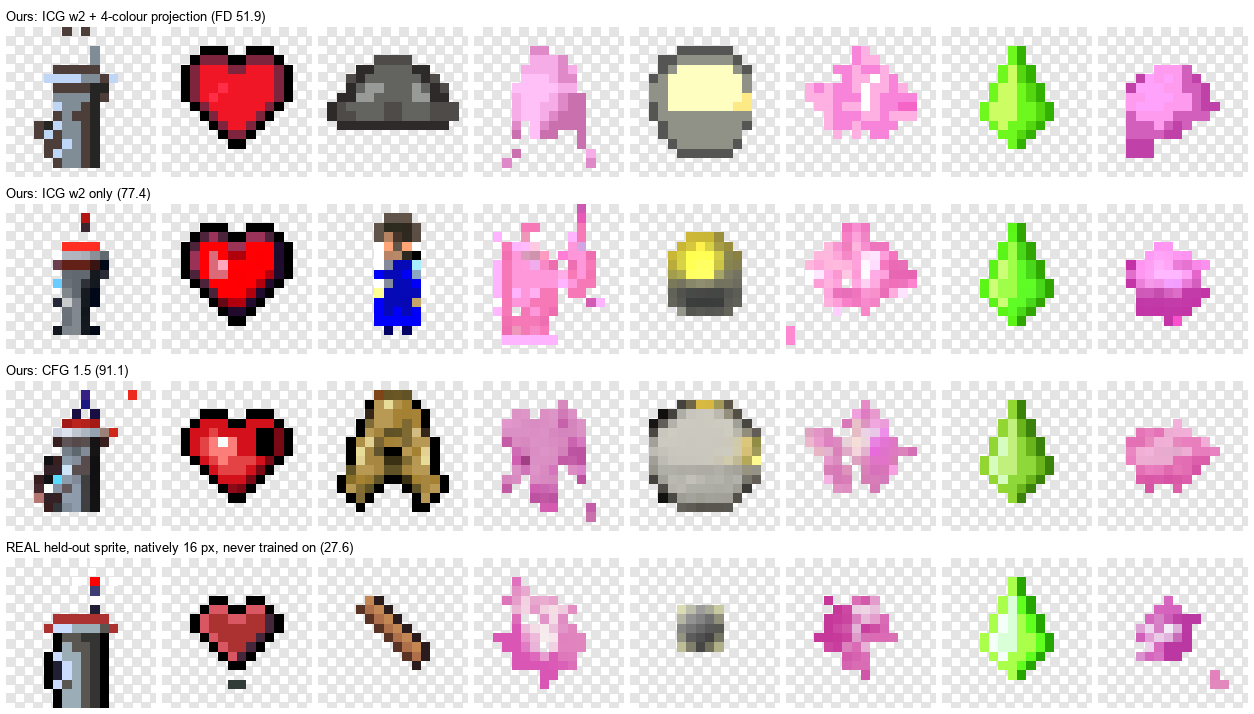
\includegraphics[width=\linewidth]{figures/fig_native_gt.png}
\caption{Twelve prompts from the training-excluded native set (sprites drawn at 16\,px and removed from training).
Rows: \ours{}; ICG only; FLUX.2-klein with a pixel-art LoRA, downscaled; the real sprite. Numbers in the row titles are
native FD on all 210 prompts of this set, including those with near-duplicate twins in training; the text reports the
124-prompt subset without them.}
\label{fig:nativegt}
\end{figure}

\paragraph{Robustness of the evaluation.}
\emph{Near-duplicate leakage}: removing the 41.4\% of prompts whose sprite has a near-duplicate twin in training
($8\times8$ average hash) changes every number by at most 3.0 FD and no ordering (\ours{}: 31.8 $\to$ 29.0).
\emph{Content}: restricting both reference and prompts to sprites a vision--language model labels as standalone objects
gives 37.1 for \ours{} against 103.0 for ICG and 144.9 for CFG (see Content labels below). \emph{Feature space}:
Inception-v3 clean-FID preserves the ordering with smaller margins (below). \emph{Training length}: 100k and 120k steps
give 30.8 and 32.3, so the model is converged.

\paragraph{Inception features.}
Inception-v3 clean-FID \citep{Parmar2022} and KID \citep{Binkowski2018} on the same saved samples and native reference preserve the ordering:
PPS $k{=}4$ 23.79, $k{=}6$ 23.28, no projection 26.27, CFG 29.37, one corpus-wide palette 36.05, median filter 66.63
(real held-out 10.54). The separation is smaller than under DINOv2 because Inception resizes its input to 299\,px,
which blurs the hard edges and flat interiors that distinguish 16\,px pixel art.

\paragraph{Content labels.}
A vision--language model labels every evaluation image (20 per numbered grid; classes object, effect, fragment, glyph,
junk). Of the 3{,}000 held-out sprites, 73.2\% are standalone objects, 15.7\% fragments, 7.8\% effects, 2.0\% glyphs and
1.3\% junk. The object-only protocol of Section~\ref{sec:analysis} keeps 825 reference sprites and 2{,}181 prompts
(\ours{} 37.1, ICG 103.0, CFG 144.9, original targets 201.3, real mixed-provenance sprites 161.3). Dropping the 8{,}818
sprites labelled fragment, glyph or junk from training improves a 20k-step run from 165.6 to 156.7 native FD; we keep
the unfiltered corpus for simplicity.

\paragraph{Training length, capacity and data scale.}
The headline model is converged: 31.8, 30.8 and 32.3 native FD at 80k, 100k and 120k steps. A $2.2\times$ larger UNet
(161.2M parameters) reaches 38.5 at 80k, so the 72.5M model is the better choice at this data scale. Adding the Kenney
CC0 packs and the OpenGameArt CC-BY-3.0 bundle (118{,}378 training rows) improves a 20k-step run from 54.2 to 42.9 but
gives $39.3\pm0.3$ at 80k against $31.8\pm0.5$ for the main corpus. Because both the capacity and the data-scale
comparisons reorder between 20k and 80k steps, every headline number in this paper is measured at full training length.
Replacing CLIP ViT-B/32 with ViT-L/14 as the text encoder gives 164.0 against 165.6 at 20k steps.

\paragraph{Quality conditioning.}
A vision--language model rates each sprite's craft from 1 to 5, and we train a separate model with the rating prepended
to the caption as a tag. Asking for the top tag at sampling time produces visibly more finished sprites
(Figure~\ref{fig:qualtag}). Because the tag concentrates the output on the best-rated 8\% of the corpus, which is
dominated by items and characters, distributional scores against the full native reference increase: the tag-trained
model scores 45.6 with the top tag and 34.2 without it, against 31.8 for the main model. We therefore keep the main model
unconditioned and offer the tag as a practitioner's control.

\begin{figure}[h]
\centering
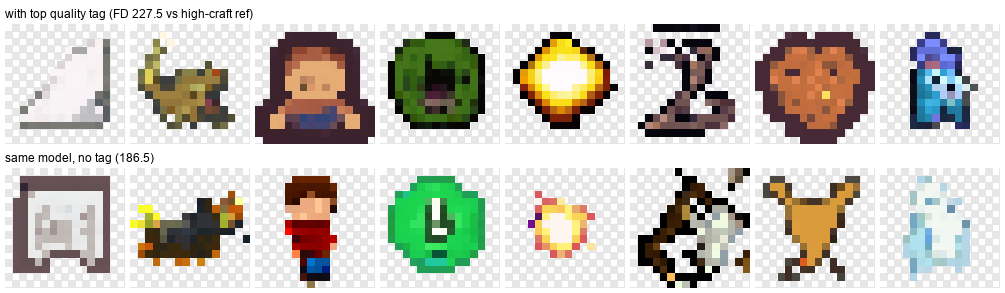
\includegraphics[width=\linewidth]{figures/fig_quality_tag.png}
\caption{Quality conditioning at 16\,px: same model, prompts and seed, sampled with (top) and without (bottom) the top
craft tag.}
\label{fig:qualtag}
\end{figure}

\paragraph{Vision--language model as a judge.}
We also put 560 forced-choice pairs over 40 captions to a vision--language model, with real held-out sprites in the pool
as a control. \ours{} ties with the real sprites (50\%) under two different question wordings. The judge, however, also
prefers the polished renders of FLUX.2 and gpt-image-2 over real sprites (72\% and 70\%), which indicates that a
general-purpose vision model responds to polish rather than to whether an image was authored at sprite resolution; this
is the property the native reference set is designed to capture, and it is why we do not use such a judge as a
substitute for a human study.

\paragraph{Canvas occupancy.}
Real sprites drawn at 16\,px cover 26\% of their canvas, while sprites that are resized to fill a bucket cover about
40\%; \ours{} covers 34\%. Preserving each sprite's native margin during bucketing is a simple extension that we leave to
future work.
